
\documentclass[a4paper,12pt]{article}
\usepackage{epstopdf}
\usepackage[utf8]{inputenc}
\usepackage[english]{babel}
\usepackage{enumerate}
\usepackage{mathtools}
\usepackage{hyperref}
\usepackage{float}
\usepackage[pdftex]{graphicx}   
\usepackage{multirow}
\usepackage{listings}
\lstset{
    language=matlab,
    basicstyle=\ttfamily
}

\title{TBMI26  \\
       Assignment 1}
\author{Martin Estgren \texttt{<mares480>}}
      
\begin{document}
 \pagenumbering{arabic}
    \maketitle % Generate.

\section{Assignment 1}

\subsection{Overview of the data}

  
Looking at the data from a machine learning perspective we can observe how the data is compressed from $32*32$ bitmap images to $64$ features with the integer range 0..16. This means that we can create a hypercube feature space with 64 dimensions. We have not lost any information but the number of dimensions have significantly decreased ($32*32 * 1 = 1024$ and $64*16 = 1024$).

The pre-processing of the data doesn't reduce the information in the data set but make it less noisy by introducing some feature-invariance.

\subsection{Implementation of the kNN algorithm}

\subsubsection{kNN without cross-validation}
The implementation of kNN is fairly straight forward. 

We iterate though all the cases in the test set and calculate the distance to each point in the training set. The result is then sorted in ascending order and the \textit{k} first elements are counted in regards to what label they are assigned. The label with the most values are then picked to be assigned for the testing case we are currently processing. When no counted label is higher than another we pick the label with the data point which have the closest euclidean distance to the test case.

The result of our implementation of the kNN algorithm with k arbitrarily chosen as 4 can be seen below.

\begin{enumerate}
\item k = 4
\item Accuracy = 0.9710
\end{enumerate}

\begin{verbatim}
cM =

    99     0     0     0     0     0     0     0     0     0
     0    97     1     0     0     0     0     0     2     3
     0     0    97     0     0     0     0     0     0     1
     0     1     0    98     0     0     0     0     0     3
     0     1     0     0    96     0     0     0     0     2
     0     0     0     1     0   100     0     0     0     1
     1     0     0     0     0     0   100     0     0     0
     0     0     2     0     0     0     0   100     0     0
     0     1     0     0     1     0     0     0    96     2
     0     0     0     1     3     0     0     0     2    88
\end{verbatim}

\begin{figure}[H]
\centering
\caption{Result from kNN}\label{fig:kNN-result}
  \begin{minipage}[]{1\textwidth}
  \includegraphics[width=\textwidth]{figures/kNN_simple.png}
  \end{minipage}
\end{figure}

\subsubsection{kNN with n-fold cross validation}

For the cross validation version the n-fold cross validation algorithm was used to determine the best value for k. For all of the following results $n = 2$ was used but the algorithm implementation allow for any value of n as long as it can evenly distribute the dataset. Accuracy is used as the validation score in order to find the best value for k.


\noindent \textbf{Dataset 1}

\textbf{Best parameters:}
\begin{itemize}
\item $k = 1$
\item $Accuracy = 0.9900$
\end{itemize}

\begin{figure}[H]
\centering
  \begin{minipage}[]{0.49\textwidth}
  \caption{Cross validation score}\label{fig:kNN-1-cv-score}
  \includegraphics[width=\textwidth]{figures/kNN_1_cv_score.png}
  \end{minipage}
  \begin{minipage}[]{0.49\textwidth}
  \caption{Cross validation result}\label{fig:kNN-1-cv}
  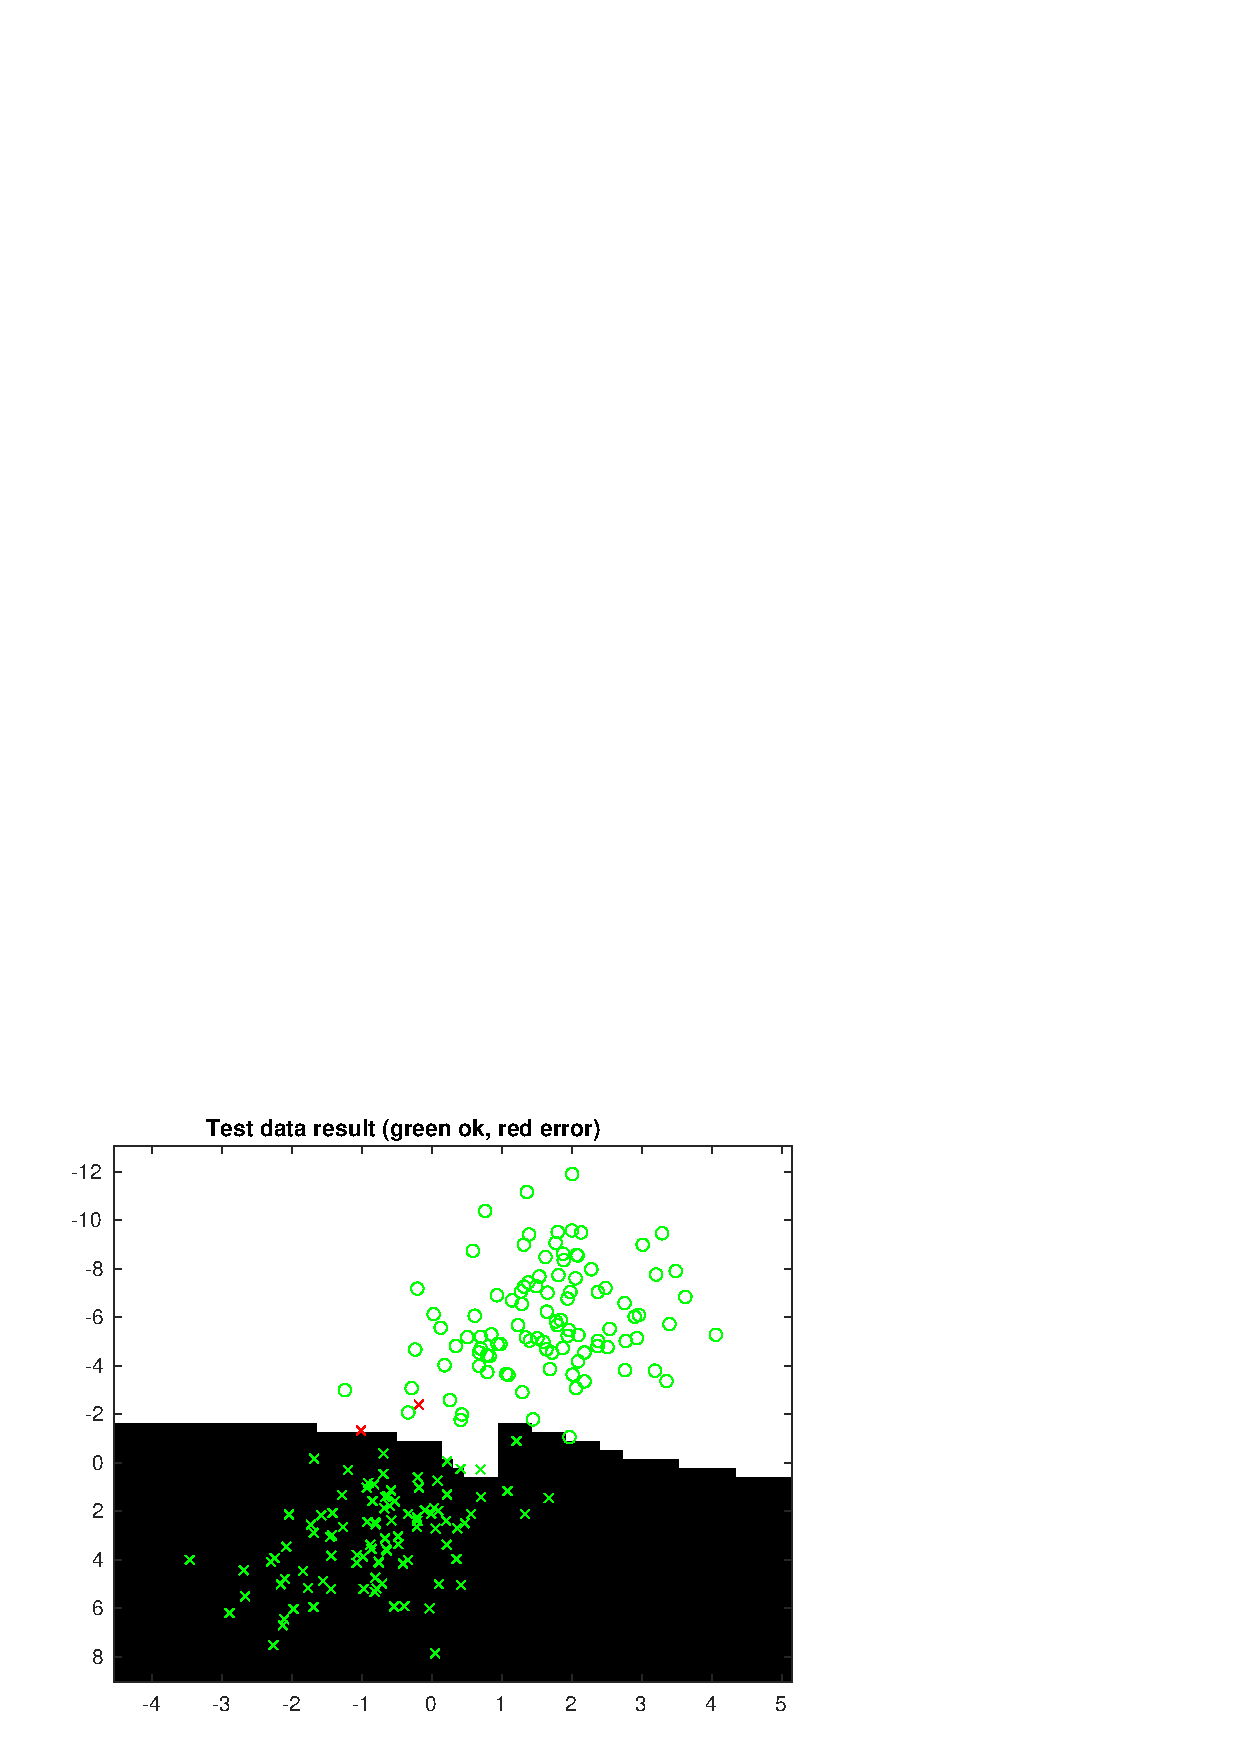
\includegraphics[width=\textwidth]{figures/kNN_1_cv.png}
  \end{minipage}
\end{figure}

\noindent \textbf{Dataset 2}

\textbf{Best parameters:}
\begin{itemize}
\item $k = 1$
\item $Accuracy = 1$
\end{itemize}

\begin{figure}[H]
\centering
  \begin{minipage}[]{0.49\textwidth}
  \caption{Cross validation score}\label{fig:kNN-2-cv-score}
  \includegraphics[width=\textwidth]{figures/kNN_2_cv_score.png}
  \end{minipage}
  \begin{minipage}[]{0.49\textwidth}
  \caption{Cross validation result}\label{fig:kNN-2-cv}
  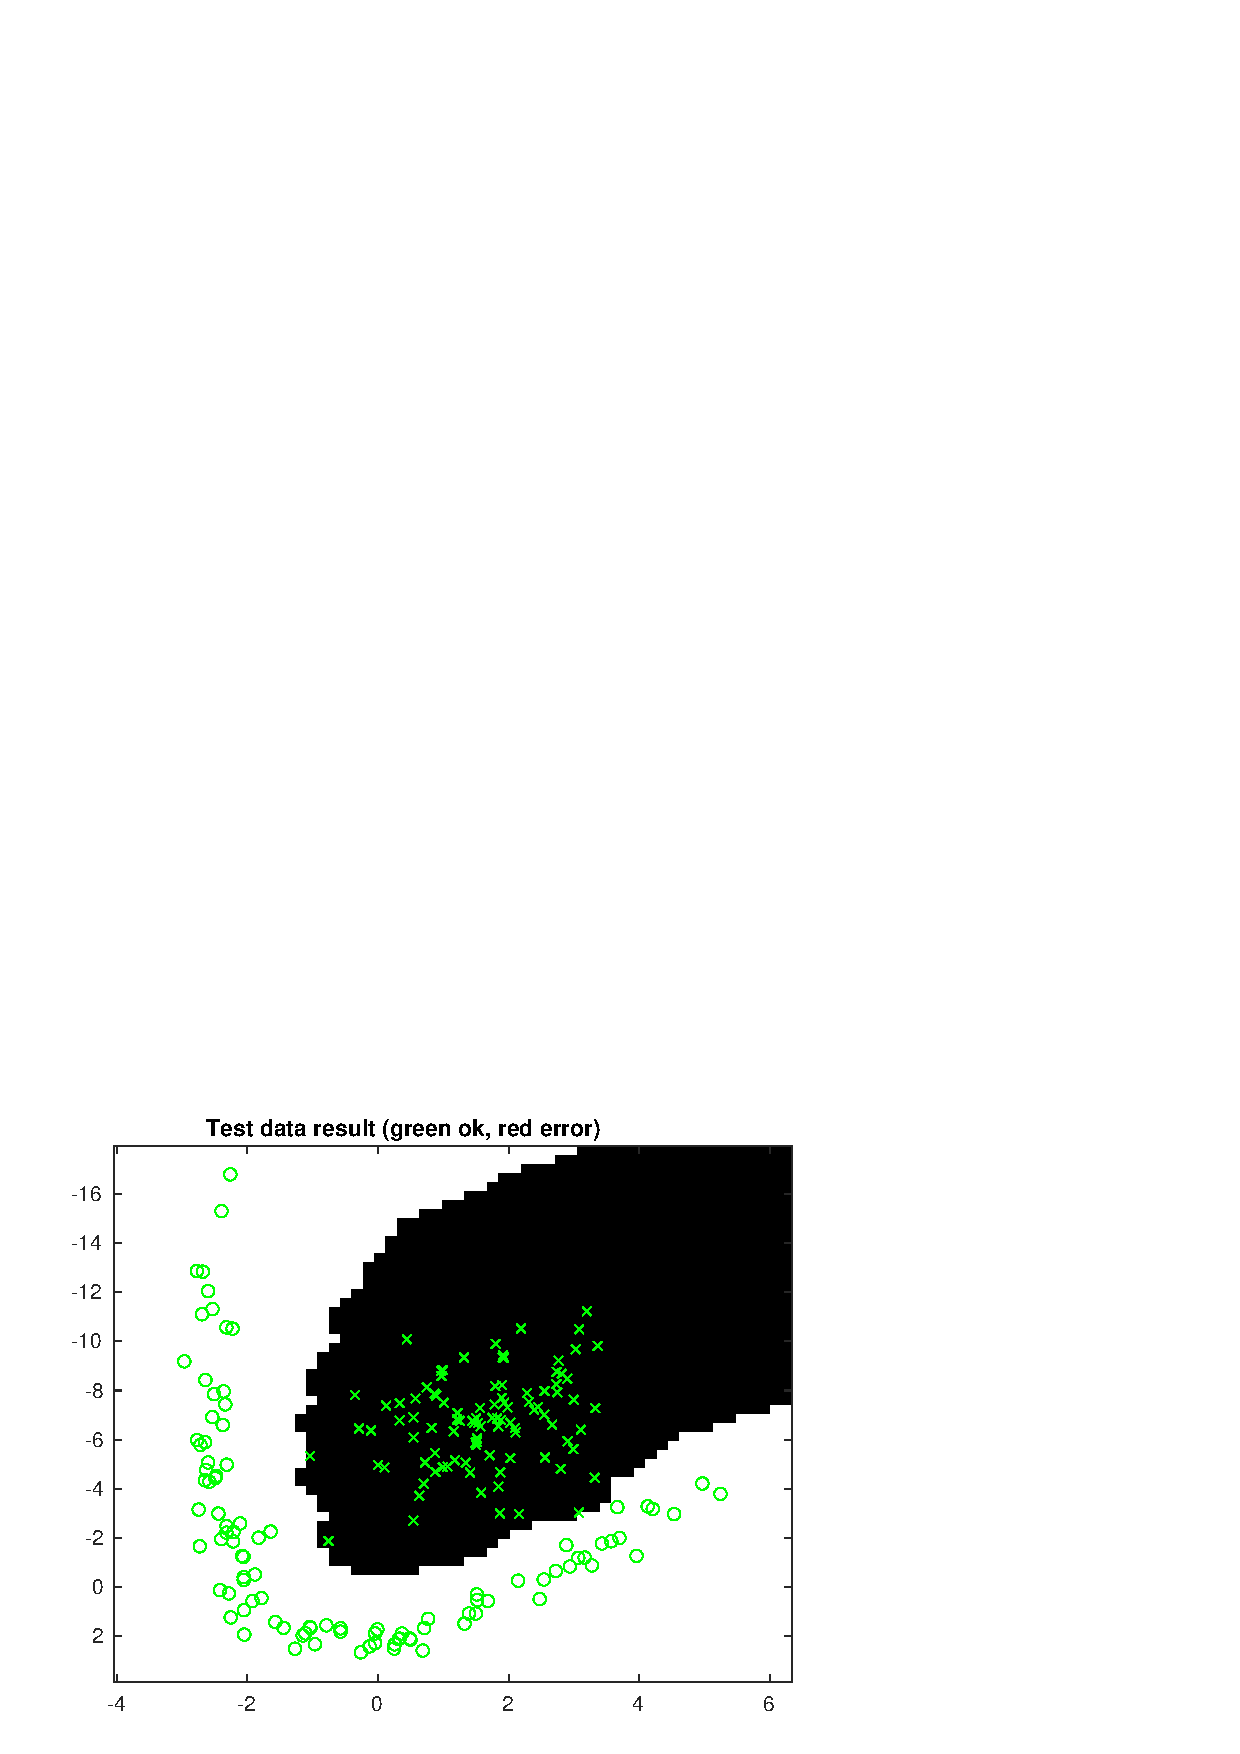
\includegraphics[width=\textwidth]{figures/kNN_2_cv.png}
  \end{minipage}
\end{figure}


\noindent \textbf{Dataset 3}

\textbf{Best parameters:}
\begin{itemize}
\item $k = 1$
\item $Accuracy = 1$
\end{itemize}

\begin{figure}[H]
\centering
  \begin{minipage}[]{0.49\textwidth}
  \caption{Cross validation score}\label{fig:kNN-3-cv-score}
  \includegraphics[width=\textwidth]{figures/kNN_3_cv_score.png}
  \end{minipage}
  \begin{minipage}[]{0.49\textwidth}
  \caption{Cross validation result}\label{fig:kNN-3-cv}
  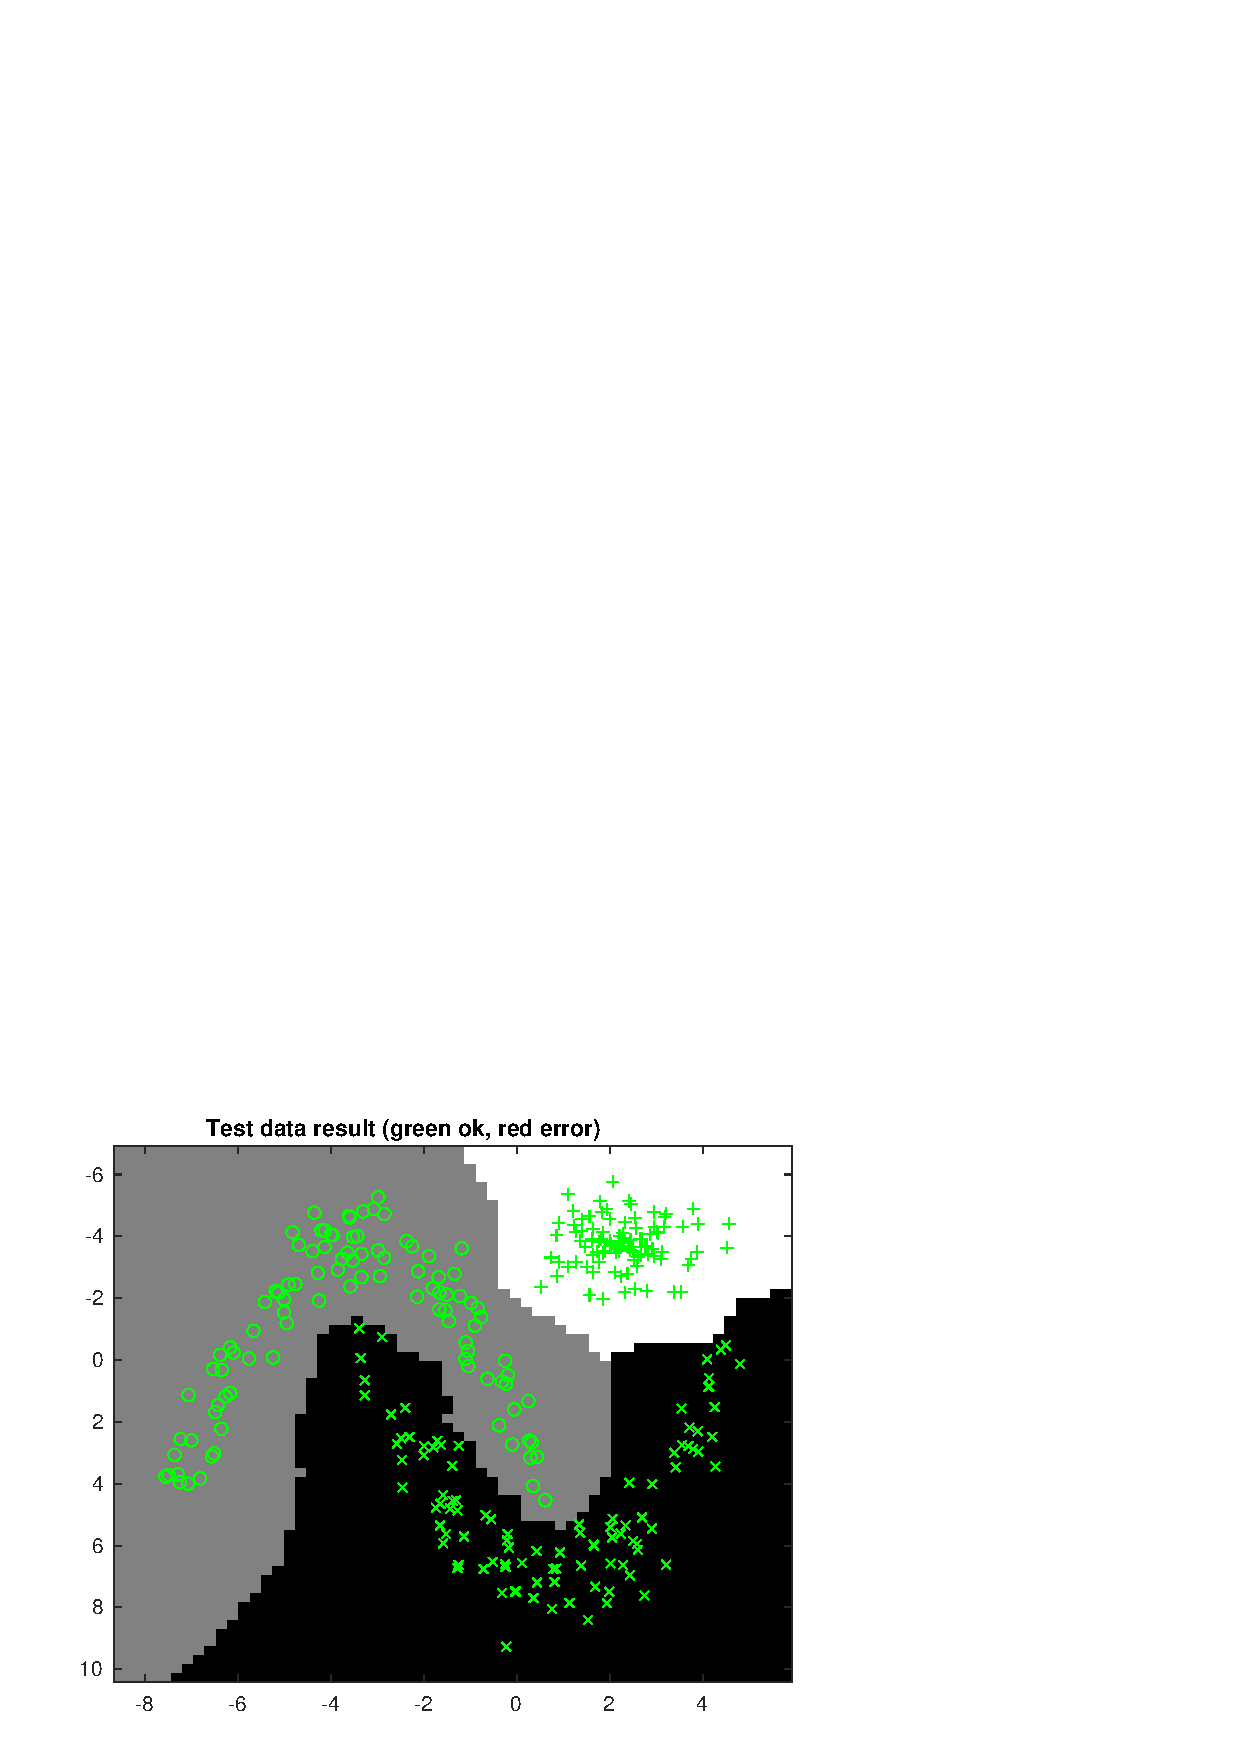
\includegraphics[width=\textwidth]{figures/kNN_3_cv.png}
  \end{minipage}
\end{figure}


\noindent \textbf{Dataset 4}

\textbf{Best parameters:}
\begin{itemize}
\item $k = 1$
\item $Accuracy = 0.9840$
\end{itemize}

\begin{figure}[H]
\centering
  \begin{minipage}[]{0.49\textwidth}
  \caption{Cross validation score}\label{fig:kNN-4-cv-score}
  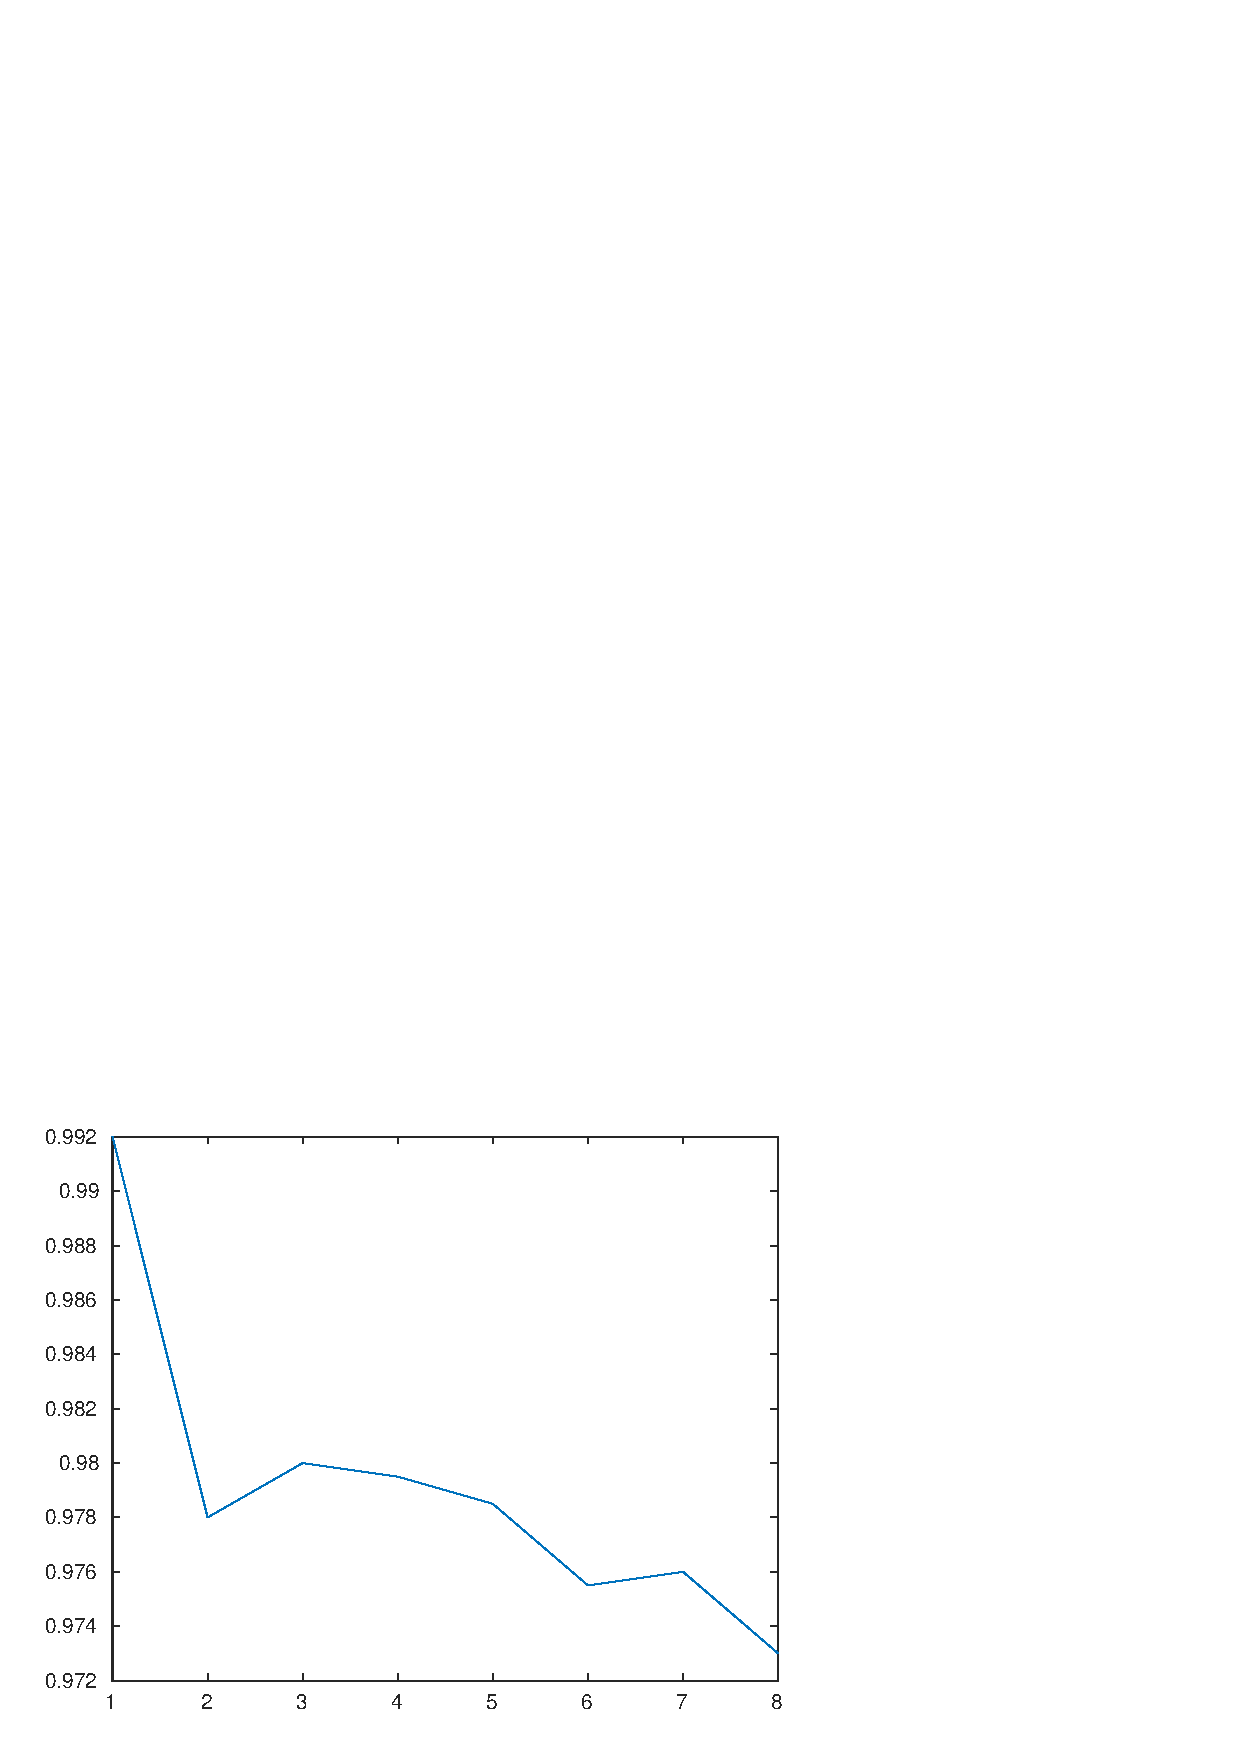
\includegraphics[width=\textwidth]{figures/kNN_4_score.png}
  \end{minipage}
  \begin{minipage}[]{0.49\textwidth}
  \caption{Cross validation result}\label{fig:kNN-4-cv}
  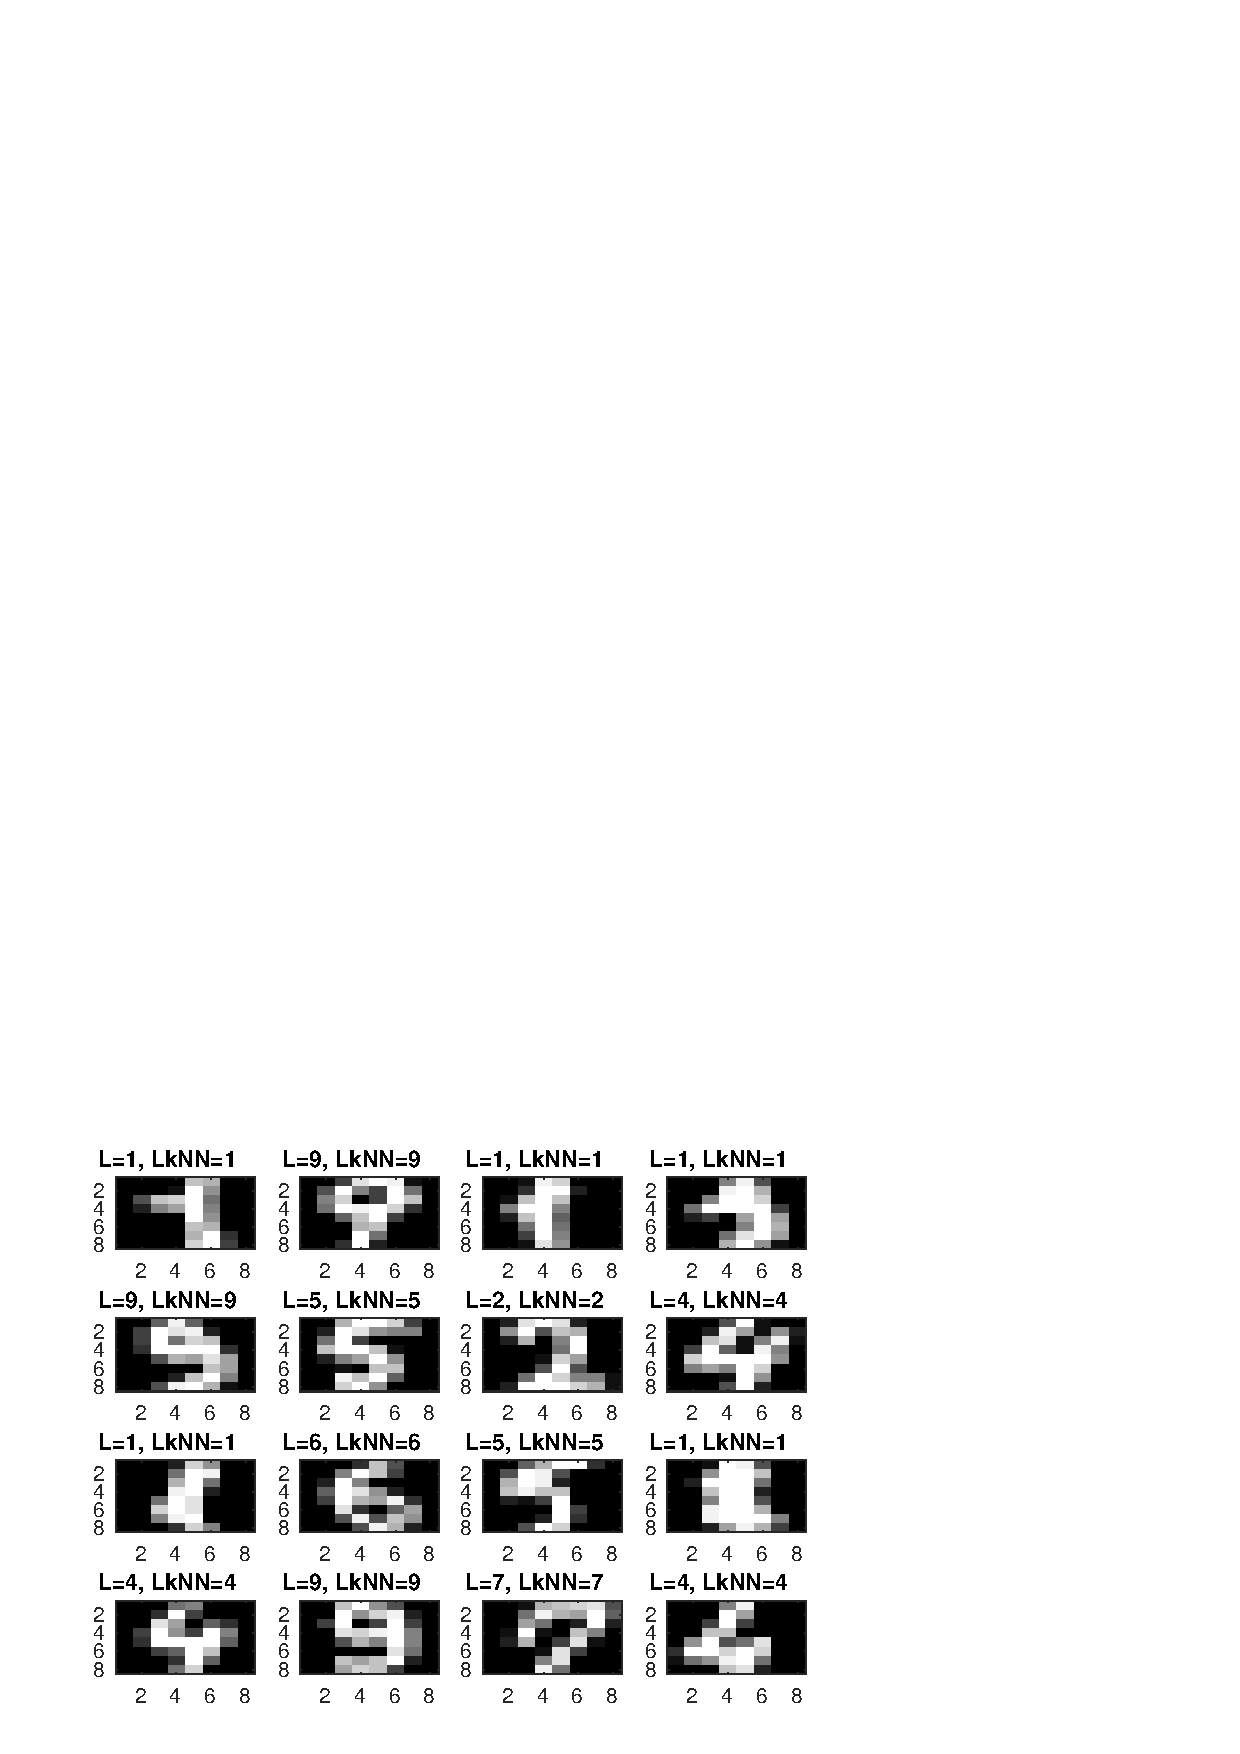
\includegraphics[width=\textwidth]{figures/kNN_4_cv.png}
  \end{minipage}
\end{figure}

\subsection{Single/Multi-layer neural network}

\subsubsection{Single layer backpropagation}

The implementation of the single layer backpropagation algorithm we use a linear activation function and the gradient $\frac{n}{s}(Y-Dt)*Xt^t$ where $n$ is the number of data to classify, $Y$ is the result from the forward propagation, $Dt$ is the expected value for $Y$ and $Xt$ is a matrix with all training features. To train the network we use backpropagation with gradient descent, meaning we calculate the gradient for our output layer and use it together with our previous weights and classification error to fine-tune our weights for better classification.


\noindent \textbf{Dataset 1}

The classification bound of this data set is not very complex which means we don't need to find the perfect weights for the neurons. In turn it will be trained in no significant time.

\textbf{Parameters:}
\begin{itemize}
\item $Iterations = 800$
\item $learning rate = 0.005$
\item $Accuracy = 0.9950$
\end{itemize}
\begin{figure}[H]
\centering
  \begin{minipage}[]{0.49\textwidth}
  \caption{Single-layer network error}\label{fig:single_1_error}
  \includegraphics[width=\textwidth]{figures/single_1_error.png}
  \end{minipage}
  \begin{minipage}[]{0.49\textwidth}
  \caption{Single-layer network result}\label{fig:single_1_test}
  \includegraphics[width=\textwidth]{figures/single_1_test.png}
  \end{minipage}
\end{figure}

\noindent \textbf{Dataset 2}

For this dataset we require much more precision which is why we increase the number of iterations and reduced the learning rate.

\textbf{Parameters:}
\begin{itemize}
\item $Iterations = 200000$
\item $learning rate = 0.00005$
\item $Accuracy = 0.8200$
\end{itemize}

\begin{figure}[H]
\centering
  \begin{minipage}[]{0.49\textwidth}
  \caption{Single-layer network error}\label{fig:single_2_error}
  \includegraphics[width=\textwidth]{figures/single_2_error.png}
  \end{minipage}
  \begin{minipage}[]{0.49\textwidth}
  \caption{Single-layer network result}\label{fig:single_2_test}
  \includegraphics[width=\textwidth]{figures/single_2_test.png}
  \end{minipage}
\end{figure}

\noindent \textbf{Dataset 3}

These parameters should work just fine for this dataset as well since the data set is only slightly more complex than the last one.

\textbf{Parameters:}
\begin{itemize}
\item $Iterations = 200000$
\item $learning rate = 0.00005$
\item $Accuracy = 0.8533$
\end{itemize}

\begin{figure}[H]
\centering
  \begin{minipage}[]{0.49\textwidth}
  \caption{Single-layer network error}\label{fig:single_3_error}
  \includegraphics[width=\textwidth]{figures/single_3_error.png}
  \end{minipage}
  \begin{minipage}[]{0.49\textwidth}
  \caption{Single-layer network result}\label{fig:single_3_test}
  \includegraphics[width=\textwidth]{figures/single_3_test.png}
  \end{minipage}
\end{figure}

\noindent \textbf{Dataset 4}

This dataset is much more complex compared to the other three but we are still dealing with the same number of neurons. We have already seen that this learning rate and iterations result in finding the optimal weights for the parameters.

\textbf{Parameters:}
\begin{itemize}
\item $Iterations = 200000$
\item $learning rate = 0.00005$
\item $Accuracy = 0.9160$
\end{itemize}

\begin{figure}[H]
\centering
  \begin{minipage}[]{1\textwidth}
  \caption{Single-layer network error}\label{fig:single_4_error}
  \includegraphics[width=\textwidth]{figures/single_4_error.png}
  \end{minipage}
\end{figure}

\begin{figure}[H]
\centering
  \begin{minipage}[]{1\textwidth}
  \caption{Single-layer network result}\label{fig:single_4_test}
  \includegraphics[width=\textwidth]{figures/single_4_test.png}
  \end{minipage}
\end{figure}


\subsubsection{Multi-layer backpropagation}

When dealing with multi layer networks we have to take care of order-of-magnitudes more number of weights. Because of this we want to limit the number of hidden neurons as much as we can. We are also using a non-linear activation function for the hidden layer which means we get transformed information at the linear output layer. As with the single-layer model we train the network using backpropagation with gradient descent. For this model we require a more elaborate gradient than the single-layer one since we have a hidden layer with non-linear activation function. To tune the hidden weights we also need to take the output layer into account, creating a chained partial derivative where both the derivative of $tanh$ and a linear function is important.

The hidden layer gradient:

\begin{equation}
\frac{2}{n}((V^T(Yt - Dt).*tanh'(W*Xt))*Xt^T)
\end{equation}
where $V$ is the weights for the output payer and $W$ is the weights for the hidden layer.

\noindent \textbf{Dataset 1}

This is a fairly simple dataset to classify with a low number of features and a linear discrimination bound already existing in feature space we only need a small number of hidden neurons.

\textbf{Parameters:}
\begin{itemize}
\item $Hidden = 5$
\item $Iterations = 2000$
\item $learning rate = 0.01$
\item $Accuracy = 0.9950$
\end{itemize}

\begin{figure}[H]
\centering
  \begin{minipage}[]{0.49\textwidth}
  \caption{Multi-layer network error}\label{fig:multi_1_error}
  \includegraphics[width=\textwidth]{figures/multi_1_error.png}
  \end{minipage}
  \begin{minipage}[]{0.49\textwidth}
  \caption{Multi-layer network result}\label{fig:multi_1_test}
  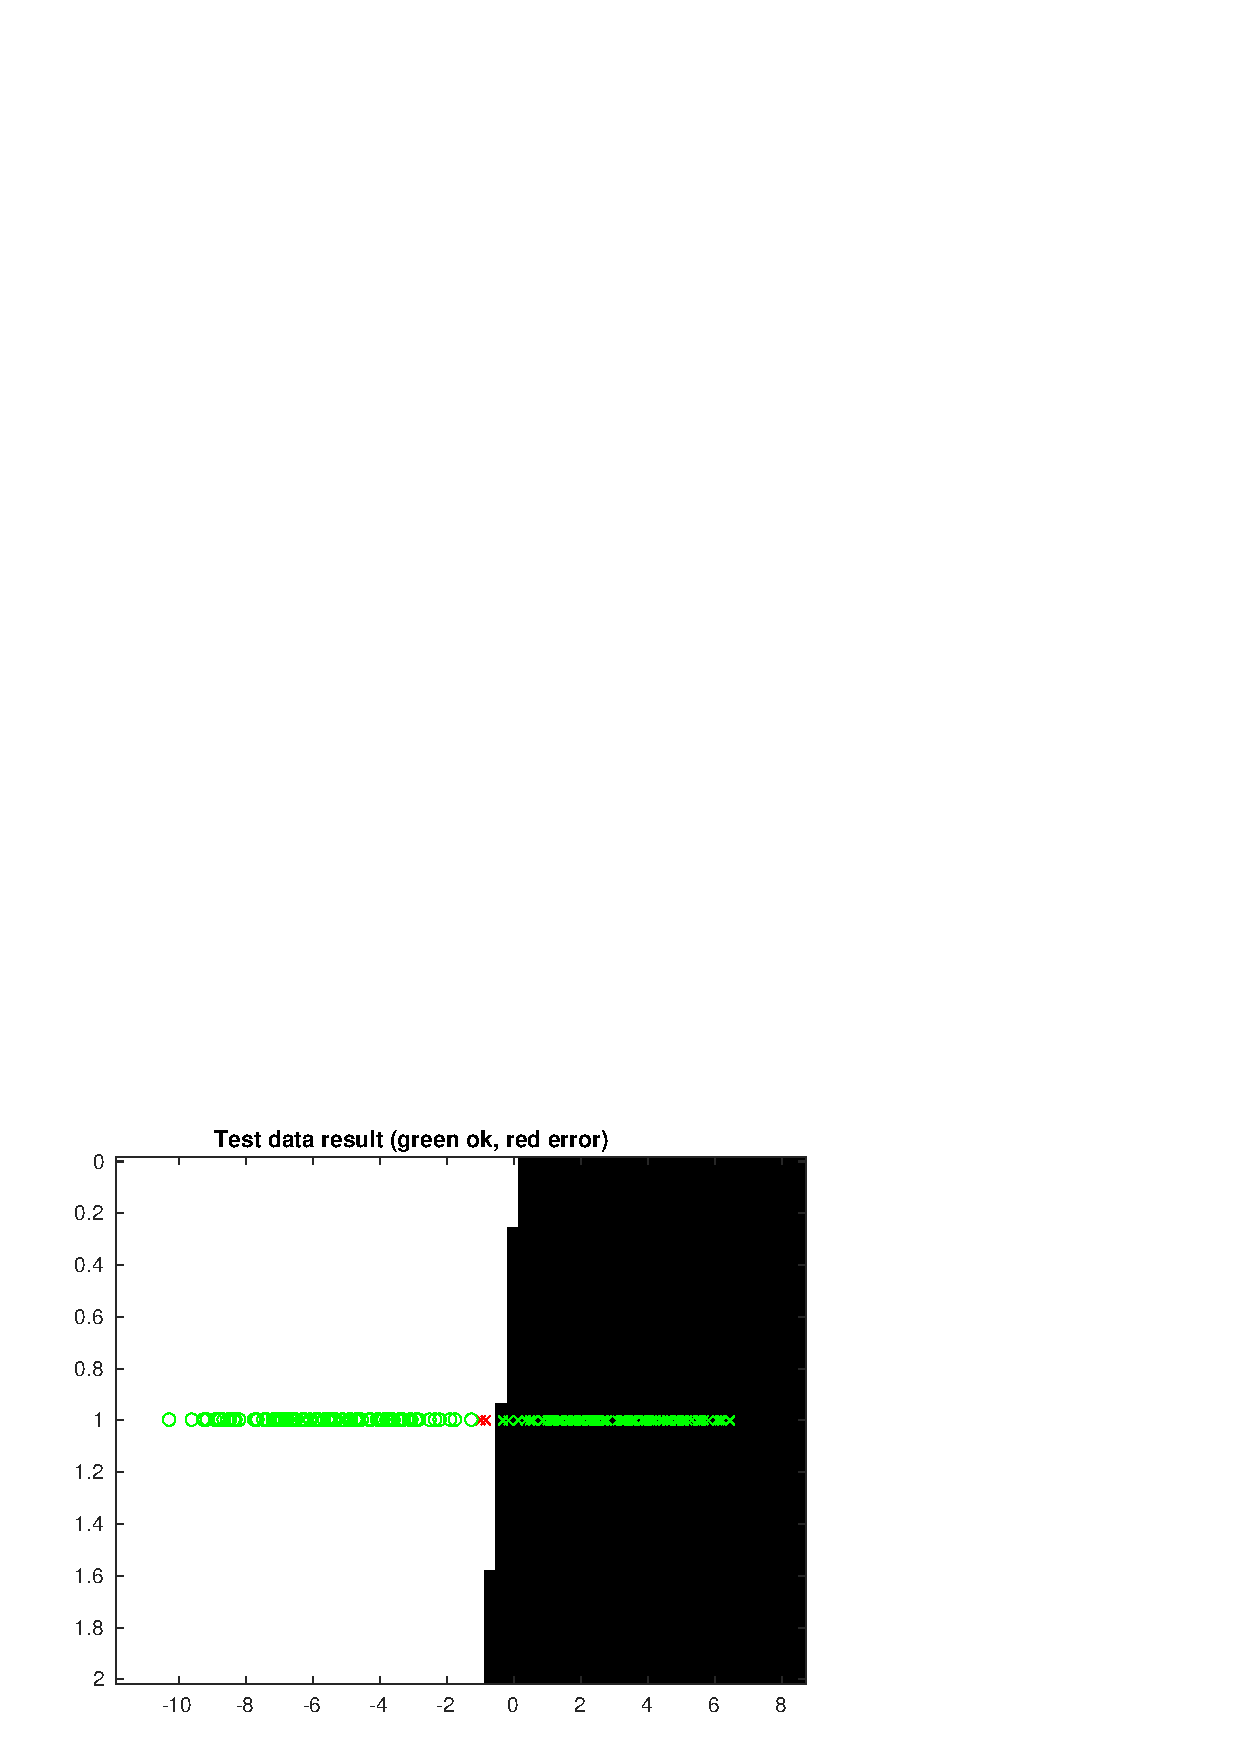
\includegraphics[width=\textwidth]{figures/multi_1_test.png}
  \end{minipage}
\end{figure}

\noindent \textbf{Dataset 2}

As with the previous dataset we have a low number of features and a fairly similar complexity for the discrimination bound. We can in this case produce a accurate representation with even fewer hidden nodes bit with a higher amount of iterations and a lower learning rate.

\textbf{Parameters:}
\begin{itemize}
\item $Hidden = 2$
\item $Iterations = 30000$
\item $learning rate = 0.005$
\item $Accuracy = 1$
\end{itemize}

\begin{figure}[H]
\centering
  \begin{minipage}[]{0.49\textwidth}
  \caption{Multi-layer network error}\label{fig:singlemulti_2_error}
  \includegraphics[width=\textwidth]{figures/multi_2_error.png}
  \end{minipage}
  \begin{minipage}[]{0.49\textwidth}
  \caption{Multi-layer network result}\label{fig:multi_2_test}
  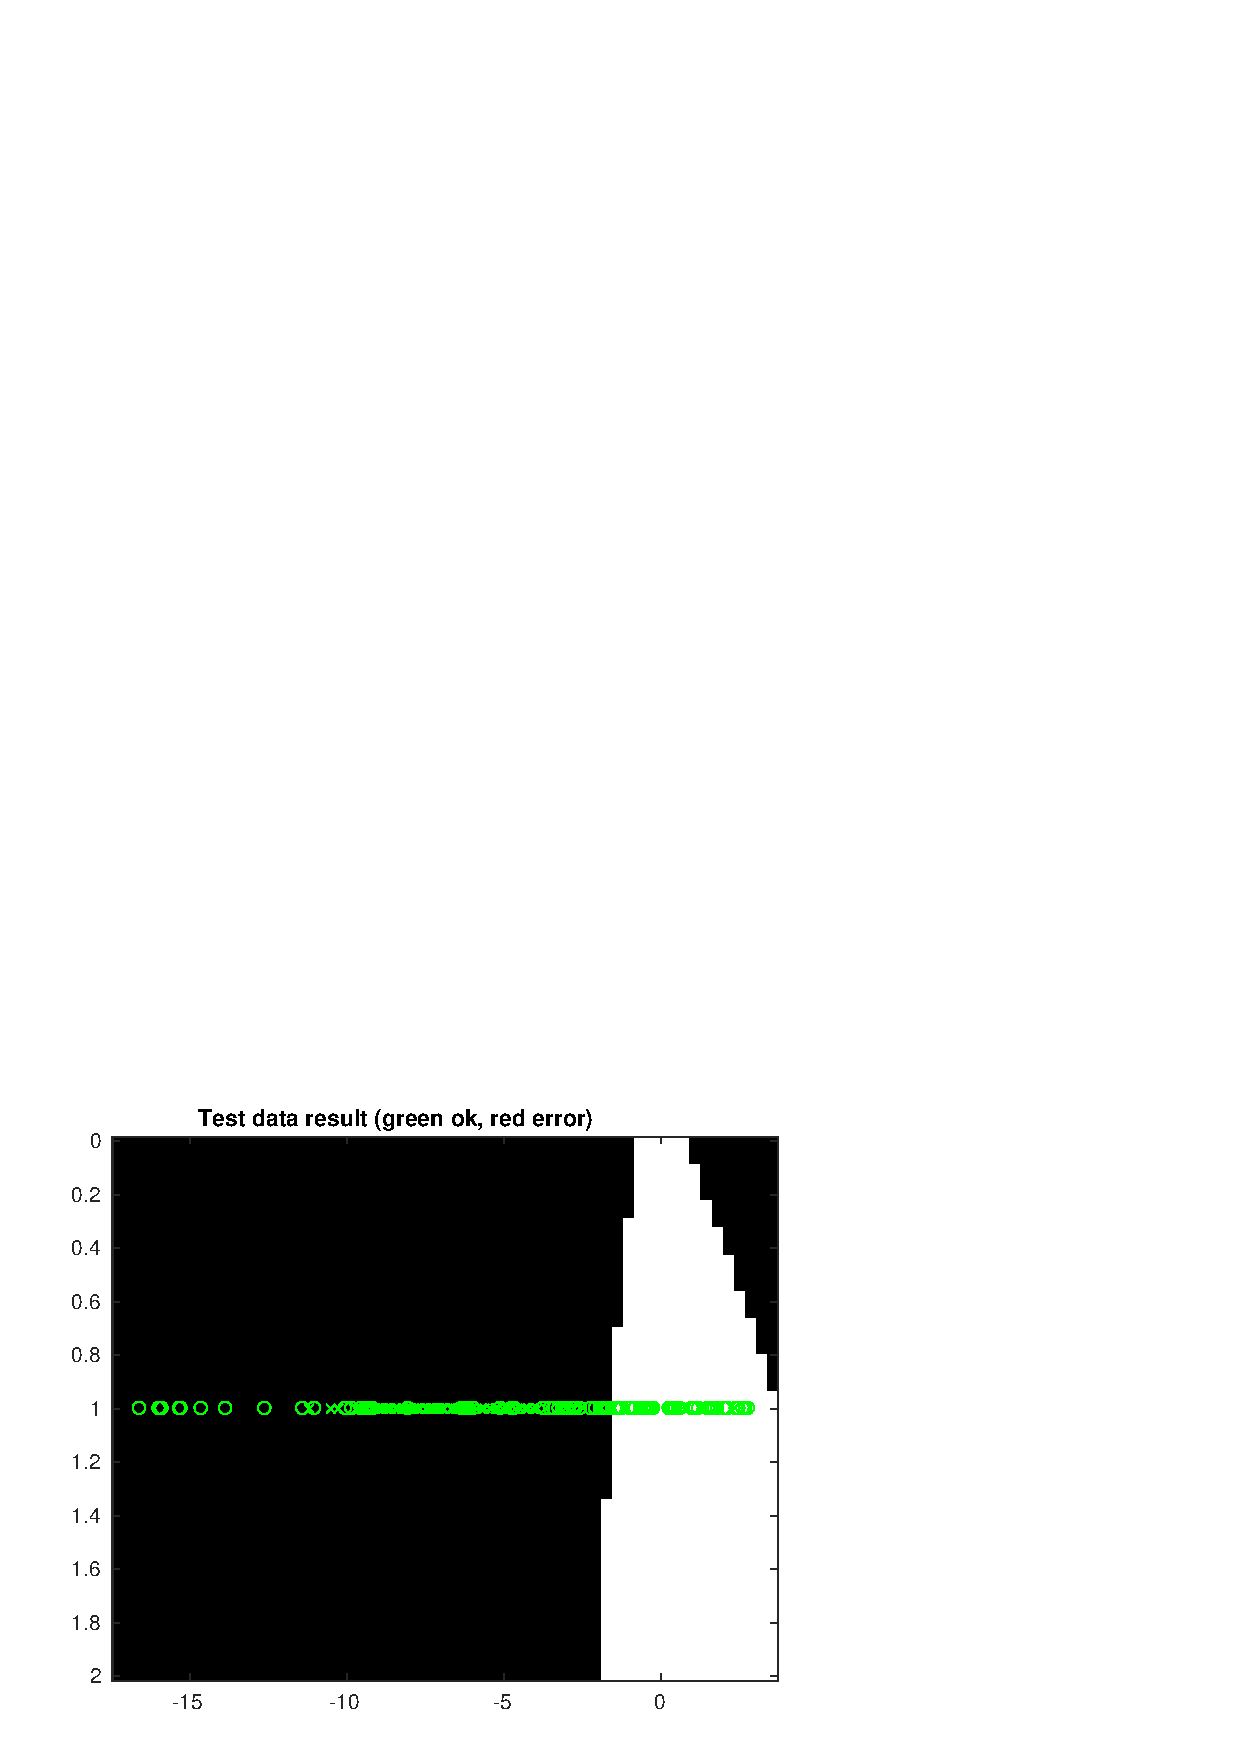
\includegraphics[width=\textwidth]{figures/multi_2_test.png}
  \end{minipage}
\end{figure}

\noindent \textbf{Dataset 3}

We are now dealing with a more complex feature space, both in terms of features and discrimination bound. Therefore we add a couple of hidden nodes and use a very small learning rate.

\textbf{Parameters:}
\begin{itemize}
\item $Hidden = 10$
\item $Iterations = 4000$
\item $learning rate = 0.005$
\item $Accuracy = 0.9967$
\end{itemize}

\begin{figure}[H]
\centering
  \begin{minipage}[]{0.49\textwidth}
  \caption{Multi-layer network error}\label{fig:multi_3_error}
  \includegraphics[width=\textwidth]{figures/multi_3_error.png}
  \end{minipage}
  \begin{minipage}[]{0.49\textwidth}
  \caption{Multi-layer network result}\label{fig:multi_3_test}
  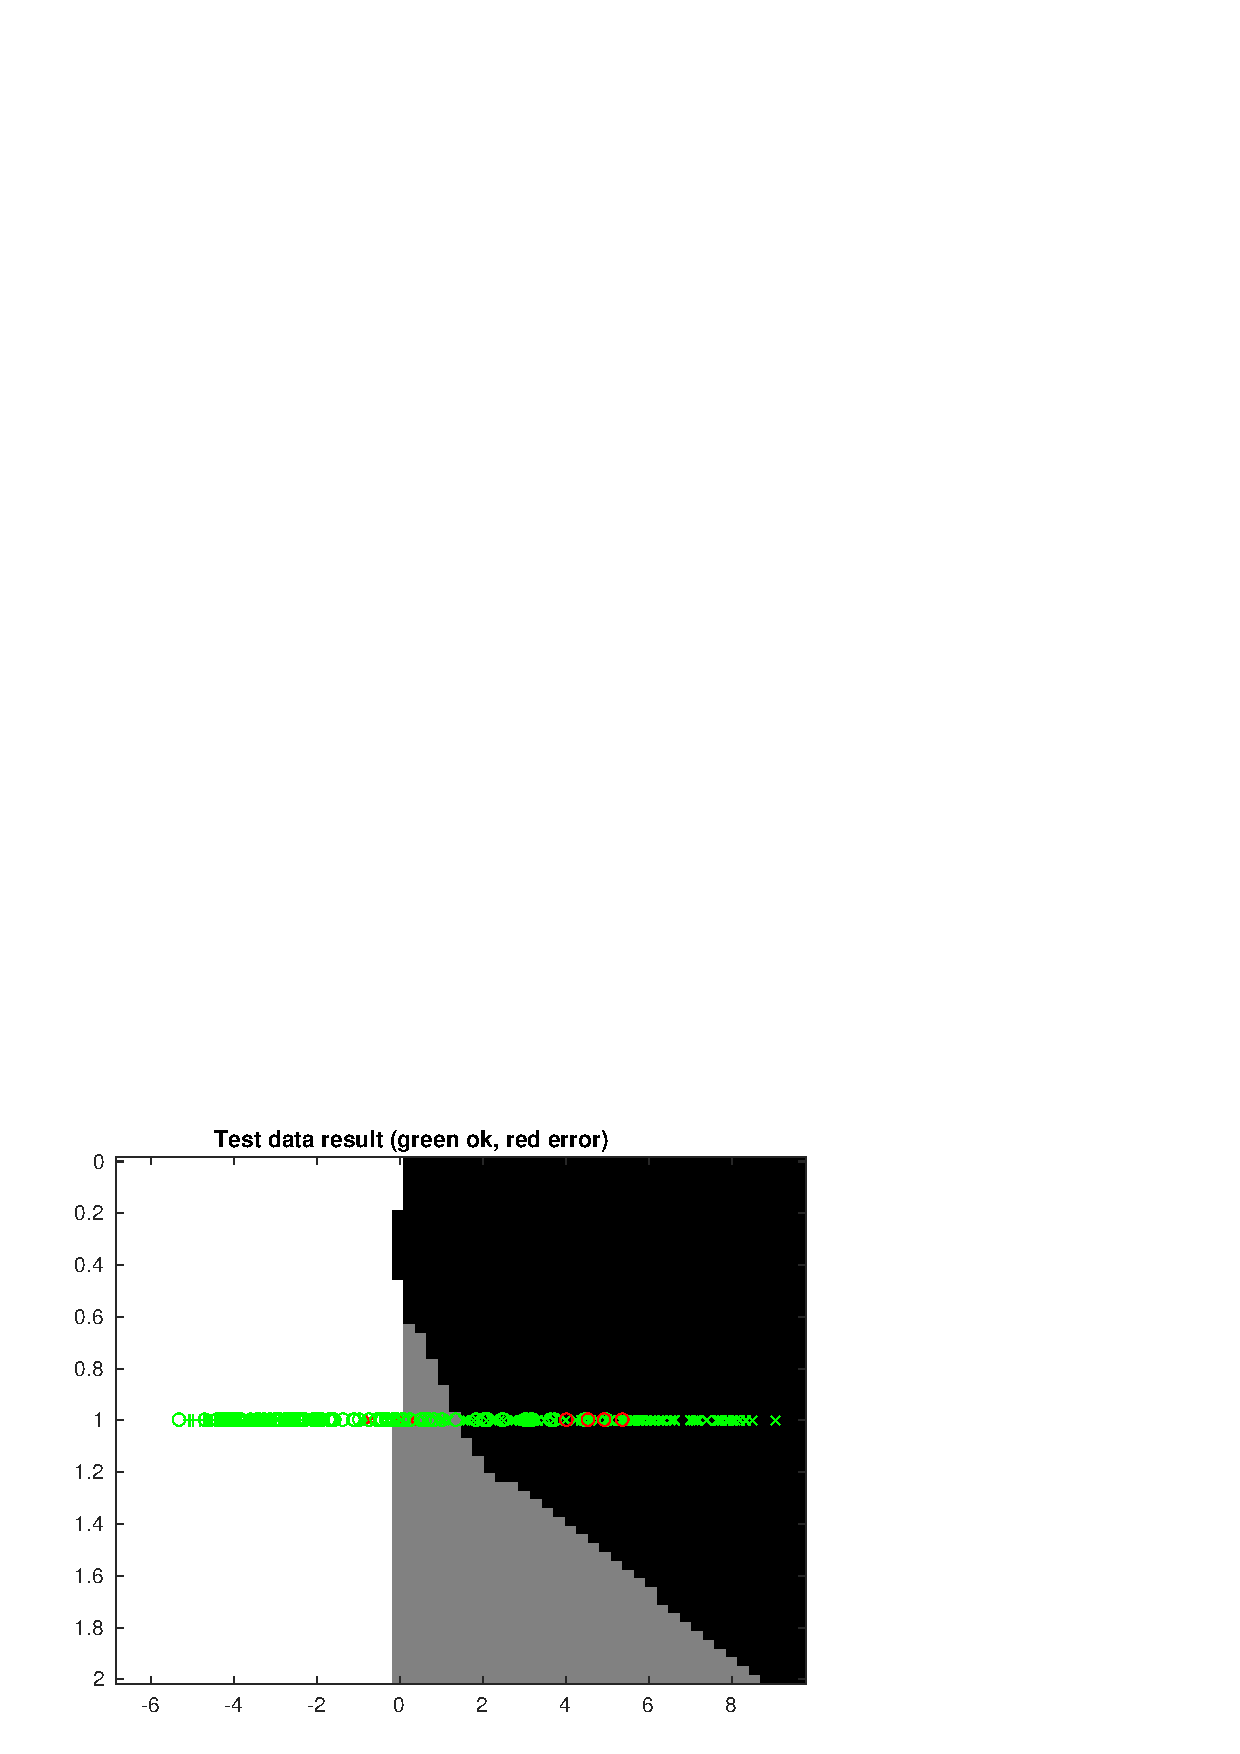
\includegraphics[width=\textwidth]{figures/multi_3_test.png}
  \end{minipage}
\end{figure}

\noindent \textbf{Dataset 4}

This dataset is a bit different, we are not dealing with only two or three dimension but 64. We also deal with more values for each features and therefore we dramatic increase the number of hidden nodes. Thought rigours testing we find that double the number of hidden nodes in relation to the features space creates a good enough classifier.

\textbf{Parameters:}
\begin{itemize}
\item $Hidden = 128$
\item $Iterations = 16400$
\item $learning rate = 0.01$
\item $Accuracy = 0.96498$
\end{itemize}

\begin{figure}[H]
\centering
  \begin{minipage}[]{1\textwidth}
  \caption{Multi-layer network error}\label{fig:multi_4_error}
  \includegraphics[width=\textwidth]{figures/multi_4_error.png}
  \end{minipage}
\end{figure}

\begin{figure}[H]
\centering
  \begin{minipage}[]{1\textwidth}
  \caption{Multi-layer network result}\label{fig:multi_4_test}
  \includegraphics[width=\textwidth]{figures/multi_4_test.png}
  \end{minipage}
\end{figure}

\subsubsection{Non-generalizable dataset}

If there's enough data points in order to find a reliable model for a unknown function we say that the model we get is non-generalizable. For example we limit our testing dataset to only 500 samples out of 999 with the parameters:

\begin{itemize}
\item $Hidden = 10$
\item $Iterations = 10000$
\item $learning rate = 0.02$
\item $Accuracy = 0.59059$
\end{itemize}

This training dataset is not generalizable since it doesn't contains enough data points to properly approximate a model for the true dataset. 

\begin{figure}[H]
\centering
  \begin{minipage}[]{1\textwidth}
  \caption{Multi-layer network error}\label{fig:non_generalizable_error}
  \includegraphics[width=\textwidth]{figures/non_generalizable_test.png}
  \end{minipage}
\end{figure}

\begin{figure}[H]
\centering
  \begin{minipage}[]{0.49\textwidth}
  \caption{Multi-layer network training data}\label{fig:non_generalizable_train}
  \includegraphics[width=\textwidth]{figures/non_generalizable_train.png}
  \end{minipage}
  \begin{minipage}[]{0.49\textwidth}
  \caption{Multi-layer network true data}\label{fig:non_generalizable_test}
  \includegraphics[width=\textwidth]{figures/non_generalizable_true.png}
  \end{minipage}
\end{figure}

\subsection{Performance of the different classifiers}

\textit{kNN} had a high degree of accuracy for all of the provided datasets. It's a simple algorithm which is both transparent and easy go understand. The main drawback is that it requires that you iterate thought the entire training set for each data point we want to classify, making it bad for large datasets. 

\textit{Single-layer neural network} performed great on the simple datasets but had greatly reduced performance on more complex datasets. Time-wise it required order of magnitudes less training time compared to the multi-layer neural networks but at the cost of flexibility.

\textit{Multi-layer neural network} had highly accurate results for each dataset but required huge amount of training time for the more complex datasets. The number of hidden nodes were fairly arbitrarily picked since we don't have the time to perform proper cross-validation. For both the single and multi-layer models, once we have a trained network - trained with a dataset similar to the true model we can easily classify new data points without consulting previous data points. This means that for huge datasets we have a significantly reduced total time in comparison with kNN.

\subsection{What could improve the results}

Usually when working with neural networks we try to normalize the input data before the model. This could have the potential to improve the results. We also randomly initialize the weights for the neural network models which can be replaced by ball-parking them before the training phase, in some cases significantly reducing the required model training time - which is our greatest problem with the neural networks.

\end{document}
